\begin{figure}[htbp]
\centering
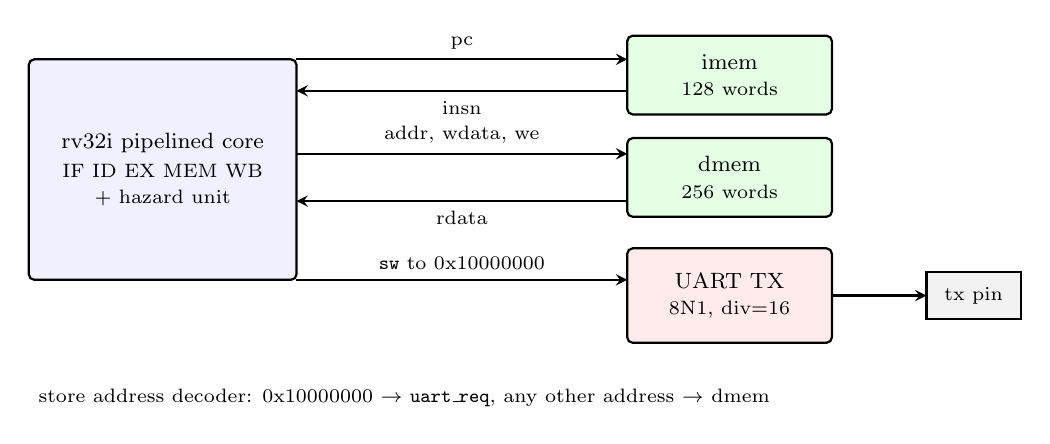
\begin{tikzpicture}[font=\footnotesize, >=stealth, x=1cm, y=1cm]
  \draw[thick, fill=blue!6, rounded corners=2pt] (0,1.0) rectangle (3.4,3.8);
  \node[align=center] at (1.7,2.4) {rv32i pipelined core\\[1pt]
    \scriptsize IF ID EX MEM WB\\ \scriptsize + hazard unit};
  \draw[thick, fill=green!10, rounded corners=2pt] (7.6,3.1) rectangle (10.2,4.1);
  \node[align=center] at (8.9,3.6) {imem\\ \scriptsize 128 words};
  \draw[thick, fill=green!10, rounded corners=2pt] (7.6,1.8) rectangle (10.2,2.8);
  \node[align=center] at (8.9,2.3) {dmem\\ \scriptsize 256 words};
  \draw[thick, fill=red!8, rounded corners=2pt] (7.6,0.2) rectangle (10.2,1.4);
  \node[align=center] at (8.9,0.8) {UART TX\\ \scriptsize 8N1, div=16};
  \draw[thick, fill=gray!10] (11.4,0.5) rectangle (12.6,1.1);
  \node at (12.0,0.8) {\scriptsize tx pin};
  \draw[->, thick] (3.4,3.8) -- node[above]{\scriptsize pc} (7.6,3.8);
  \draw[->, thick] (7.6,3.4) -- node[below]{\scriptsize insn} (3.4,3.4);
  \draw[->, thick] (3.4,2.6) -- node[above]{\scriptsize addr, wdata, we} (7.6,2.6);
  \draw[->, thick] (7.6,2.0) -- node[below]{\scriptsize rdata} (3.4,2.0);
  \draw[->, thick] (3.4,1.0) -- node[above]{\scriptsize \texttt{sw} to 0x10000000} (7.6,1.0);
  \draw[->, thick] (10.2,0.8) -- (11.4,0.8);
  \node[align=left, anchor=west, font=\scriptsize] at (0.0,-0.5)
    {store address decoder: 0x10000000 $\to$ \texttt{uart\_req}, any other address $\to$ dmem};
\end{tikzpicture}
\caption{The ch08 SoC: the pipelined core, instruction memory, data
memory, and a memory-mapped UART. One extra address-compare line
turns an ordinary \texttt{sw} into a serial transmission.}
\label{fig:soc08}
\end{figure}
